\chapter{Evaluatie}
In deze sectie wordt de ontwikkelde library ge\"evalueerd. Allereerst wordt er gekeken naar wat de impact van de library op de performance van de applicatie is. Verder in dit hoofdstuk wordt de schaalbaarheid van de library bekeken. Tot slot wordt er nog gekeken hoeveel effort er van de developer nodig is om de library te integreren in een applicatie. Uit deze evaluaties wordt een conclusie getrokken over de Tracklytics library.


\section{Performance}
In het hoofdstuk Doelstellingen is aangehaald dat impact van de Tracklytics library op de performance aanvaardbaar moet zijn om de applicatie niet significant te doen vertragen. In deze sectie wordt deze impact onderzocht en ge\"evalueerd. \\

Om de performance te meten zijn er twee verschillende applicaties gekozen waar de library in ingebouwd is, namelijk een stopwatch applicatie en een angry birds kloon \cite{AngryBirds}. De stopwatch wordt gebruikt omdat dit een niet CPU intensieve applicatie is en zo de resultaten niet vertekend zijn. De angry birds applicatie is CPU intensiever en vereist een bepaalde framerate, aangezien dit een spel is. Deze applicatie wordt gebruikt  om de impact van de Tracklytics library op de framerate te onderzoeken. \\

De evaluaties zijn uitgevoerd op een iPhone 6 \cite{iPhone} met als besturingssysteem: iOS versie 9.3.1. Het toestel was ten allen tijde voorzien van een WiFi verbinding met het internet. Om de resultaten op te halen van het toestel is de ontwikkelaarsomgeving Xcode \cite{Xcode} versie 7.3.1 gebruikt.\\

In de volgende secties worden de metingen uitgelegd en uitgevoerd. Er gaat gemeten worden hoe lang de gemiddelde uitvoeringstijd bedraagt per methode die gebruikt kan worden van de library. Nadien wordt er gekeken naar de impact van de library op de framerate van de angry birds kloon.\\

\subsection{Call duration}
In deze sectie wordt uitgezocht hoelang het gemiddeld duurt voor elke methode om volledig uitgevoerd te worden. Zo kan er een beeld gevormd worden van hoe sterk de library de applicatie zou vertragen. Om te testen hoe lang een methode gemiddeld duurt om uitgevoerd te worden, is de volgende testopstelling uitgedacht. De geteste methode wordt X aantal keer uitgevoerd om hieruit een gemiddelde tijd te kunnen berekenen. deze X wordt stelselmatig verhoogd om te kijken of de grootte van deze X een invloed heeft op de gemiddelde vertraging van de geteste methode. Deze testopstelling wordt gebruikt om alle beschikbare methodes in de Tracklytics library te evalueren. Het synchronisatieinterval is 60 seconden. \\

In de vorige secties is beschreven dat de developer de keuze gegeven is tussen het tijdelijk opslaan van de metingen op de harde schijf van het toestel en het niet opslaan van de metingen op de harde schijf van het toestel. Dit heeft een invloed op de prestaties van de library, omdat er een significant prestatieverschil zit in disk I/O en verwerkingskracht \cite{diskIO}. Om dit prestatieverschil in kaart te brengen is deze evaluatie uitgevoerd eenmaal met het opslaan op disk en eenmaal zonder het opslaan op disk (aangegeven in de resultaten als ZOD).\\

Er is in de Tracklytics library gekozen om de developer de vrijheid te geven om te beslissen dat de aggregatie van de metingen deels op het toestel van de gebruiker uitgevoerd wordt of dat deze aggregatie volledig uitgevoerd wordt in de back end. Omdat er een verschil is in de implementatie van de geaggregeerde meetobjecten en de standaard meetobjecten zijn de testen opgedeeld in testen voor de standaard meetobjecten en testen voor de geaggregeerde meetobjecten (in het geval van de Gauge, de Meter en de Timer). Zo kunnen er de juiste conclusies getrokken worden uit de testen die uitgevoerd zijn.\\


De resultaten van het testen van de standaard meetobjecten kunnen gevonden worden in volgende tabellen: \ref{Table:Counter}, \ref{Table:Gauge}, \ref{Table:Histogram}, \ref{Table:Meter}, \ref{Table:Timer}. De resultaten van de testen op de geaggregeerde meetobjecten zijn opgelijst in volgende tabellen: \ref{Table:GaugeAggregate}, \ref{Table:MeterAggregate}, \ref{Table:TimerAggregate}. De conclusies die uit deze resultaten getrokken kunnen worden zijn beschreven in de conclusie sectie \ref{Section:Conclusie}. \\


Om een vergelijking te geven van het verschil in duratie tijd van het opslaan op harde schijf en het niet opslaan op harde schijf zijn deze in grafieken samengevat: \ref{fig:GraphCounter}, \ref{fig:GraphCounterInc}, \ref{fig:GraphCounterDec}, \ref{fig:GraphTimer}, \ref{fig:GraphTimerStop}, \ref{fig:GraphTimerAggregate}, \ref{fig:GraphTimerAggregateStop}, \ref{fig:GraphHistogram}, \ref{fig:GraphMeter}, \ref{fig:GraphMeterAggregate}, \ref{fig:GraphGauge}, \ref{fig:GraphGaugeAggregate}. Met behulp van deze grafieken is de evolutie van de duratie tijd zichtbaar. 

\subsection{Invloed op FPS}
De gemiddelde tijd om een methode uit te voeren zegt iets over de vertraging die de library extra invoert in de applicatie. Het zegt echter niets over de impact op de framerate van de applicatie. Om dit te kunnen testen is er gekozen om de impact van de library op een game te testen. Zoals eerder vermeldt is deze game een angry birds kloon. \\

Om deze test uit te voeren is de volgende testopstelling gebruikt. Het gemiddeld aantal frames per second (FPS) wordt berekend uit 3000 gemeten waarden. Een FPS waarde wordt elke 0.2 seconde gemeten. Om de impact van de library op deze FPS te testen is ervoor gekozen om elke seconde X aantal keer een library call uit te voeren en deze X telkens te verhogen. Er is gekozen om de worst case test uit te voeren gebaseerd op de test van de call duration. In de resultaten is te zien dat het aanmaken van het Counter object met het opslaan op disk het hoogste gemiddelde heeft. Het aanmaken van een Counter met het opslaan van de data op de harde schijf wordt gebruikt om de invloed van de library op de FPS te onderzoeken. Om de invloed van de library op de FPS van de applicatie te onderzoeken zonder dat de metingen op de harde schijf opgeslagen worden, wordt het stoppen van een Timer gebruikt, omdat deze de grootste call duratie heeft van de niet-geaggregeerde objecten. \\

Een andere factor die invloed kan hebben op de impact die de library heeft op de applicatie is het synchronisatieinterval. Dit interval is een indicatie van hoeveel tijd er tussen twee synchronisatiecycly bevindt. Door dit synchronisatieinterval systematisch te verlagen kan de invloed van de Tracklytics library op de FPS van de applicatie gemeten worden. \\

De resultaten van deze testen kunnen gevonden worden in de volgende tabellen: \ref{Table:FPS}, \ref{Table:FPSZOD}. De linkerkolom geeft het aantal simultane metingen weer. Het synchronisatieinterval wordt systematisch verlaagd van 60 seconden naar 5 seconden. De conclusies die uit deze resultaten getrokken kunnen worden zijn beschreven in de conclusie sectie \ref{Section:Conclusie}.




\section{Schaalbaarheid}
Het is belangrijk dat de Tracklytics back end een schaalbare back end is. Indien de load op de servers te groot wordt, dan zou dit merkbaar zijn in de applicatie. De Tracklytics library zou de netwerkinterface constant gebruiken om de metingen te synchroniseren naar de back end. De applicatie waarin de library is ingebouwd deelt deze netwerkinterface met de library. Als gevolg hiervan wordt de applicatie trager, omdat de netwerkinterface constant gebruikt wordt door de library. Dit scenario moet voorkomen worden om de bruikbaarheid van de Tracklytics library optimaal te houden.\\

Een oplossing voor dit probleem is de back end uit te schalen over meerdere servers en servers bij te voegen indien de load op de servers te groot wordt. Om de back end schaalbaar te maken moet zowel de PHP code die op de servers draait schaalbaar zijn, alsook de database die in de back end draait. \\

De PHP code zet verwerkt de metingen komende van de Tracklytics library en zet deze resultaten in de database. Voor deze code is het voldoende dat deze een connectie tot een database hebben en dit maakt de PHP code dus zeer schaalbaar.\\

De database gebruikt in de Tracklytics library is een MySQL database. Dit is een implementatie van een Relational database management system (RDBMS). Dit soort database is niet ontwikkeld om schaalbaar te zijn \cite{RDBMS}. Dit soort systeem is ontwikkeld om op \'e\'en server te draaien om de integriteit van de tabel mappings te behouden en de problemen van gedistribueerde verwerking te vermijden. Indien dit systeem dan geschaald moet worden, dan moet er grotere en complexere hardware gekocht worden met meer verwerkingskracht, RAM geheugen en opslag. Een oplossing die hiervoor gevonden is, is een master-slave model waarbij de slaves de load van de master kunnen verlagen \cite{MasterSlave}. \\
Een alternatief hiervoor zou zijn om een NoSQL database te gebruiken. Dit soort database is ontwikkeld om schaalbaar te zijn. Het nadeel hiervan is dat de ACID properties niet gegarandeerd kunnen worden, wat ervoor zorgt dat data inconsistent kan worden. Er bestaat ook nog geen standaard taal (zoals SQL voor RDBMS), zodat de overgang van een RDBMS (of van een andere NoSQL) naar een NoSQL database een probleem kan vormen. \\


Een alternief is dat developers van een applicatie de Tracklytics back end hosten op hun eigen servers. Dit is mogelijk, omdat de library open source is. Enkel de connectie met de database moet aangepast worden en de links in de mobiele library moeten vervangen worden door een link naar de server van de developer. Dit geeft als voordeel dat de data zich bij de developer bevindt en de developer hier eventueel andere overzichten van kan genereren, aangepast aan zijn noden. In dit scenario is de developer niet afhankelijk van een gemeenschappelijke Tracklytics back end en heeft hij de performance van de Tracklytics back end in eigen handen. Het nadeel aan dit alternatief is dat de developer zelf serverruimte moet voorzien en onderhouden om de back end op te draaien. \\


\section{Developer effort}\label{Section:Effort}
Met DevOps willen developers en managers het ontwikkelingsproces van software versnellen. Indien het relatief veel tijd inneemt om de Tracklytics library in een applicatie in te bouwen is het developer aspect verdwenen uit deze thesis. Het is ongewenst dat het veel lijnen code inneemt om de libray in de applicatie in te bouwen, omdat dit enerzijds meer tijd inneemt om de code te schrijven en anderzijds de code minder overzichtelijk maakt voor de developers. \\

Om deze eigenschappen na te gaan is ervoor gekozen om volgende zaken na te gaan: hoeveel tijd neemt het in om de library in te bouwen, het aantal lijnen code nodig om deze in de applicatie in te bouwen, wat er gemonitord wordt en hoeveel metingen er maximaal simultaan voorkomen. Met "hoeveel tijd neemt het in om de library in te bouwen"  wordt de gehele flow bedoeld: het registreren van de applicatie in de back end, het installeren van de library via CocoaPods en het implementeren van de code in de applicatie. \\

Om deze zaken na te gaan zijn er twee applicaties gebruikt, namelijk de stopwatch applicatie die eerder vermeldt is en een applicatie ontwikkeld in mijn stage. De stopwatch heeft volgende eigenschappen:
\begin{itemize}
\item 250 lijnen code
\item 13 uren ontwikkelingstijd (inclusief design)
\end{itemize} 

De tweede applicatie heeft volgende eigenschappen:
\begin{itemize}
\item \underline{+} 10000 lijnen code
\item 4 maanden ontwikkelingstijd (inclusief design)
\end{itemize}

\subsection{Resultaten}
In deze sectie worden de resultaten besproken van de evaluatie van de developer effort. In de volgende sectie worden deze resultaten besproken \ref{Section:Conclusie}.
\subsubsection{StopWatch applicatie}
\begin{itemize}
\item ​​Duratie: Minder dan 10 minuten
\item \#Lijnen code:\begin{itemize}
\item 9 meetobjecten in totaal
\item ​gemiddeld 1.0 lijnen per meetobject(zonder imports)
\item in totaal 9 lijnen extra code
\end{itemize}

\item ​​​Tracken van: alle buttons, tijd wanneer op stop gedrukt, aantal rondes alvorens reset, tijd om data van een server te halen.

\item Maximaal 2 metingen tegelijk (Counter \& Gauge)
\end{itemize}




\subsubsection{Andere applicatie}
\begin{itemize}
\item ​Duratie: \underline{+} anderhalf uur
\item \#​Lijnen code: \begin{itemize}
\item 68 meetobjecten in totaal
\item ​​gemiddeld 1.4 lijnen per meetobject (zonder imports)
\item in totaal \underline{+} 100 lijnen extra code
\end{itemize}

\item ​Tracken van: Alle buttons waarop geklikt wordt, alle screen visits, \#zoekresultaten, duratie van complexe code, duratie content van het netwerk halen
\item Maximaal \underline{+} 10 metingen tegelijk (Counters, Timers en Gauges)
\end{itemize}


Het is nuttig om dit soort informatie te meten, omdat met behulp van dit soort metingen kan ondervonden worden hoe de gebruiker de applicatie gebruikt. Er kan zo een overzicht gevormd worden welke knoppen hoe vaak gebruikt worden en welke schermen dat de gebruiker het vaakst bezoekt. Anderzijds is het monitoren van de duratie van complexe code en van het ophalen van informatie van het netwerk een manier om bottlenecks te kunnen ontdekken in de applicatie. 

\section{Conclusie en bespreking resultaten}\label{Section:Conclusie}
In het hoofdstuk Doelstellingen is er besproken dat de impact van de ontwikkelde Tracklytics library op de performance van de applicatie zo minimaal mogelijk moet zijn. Indien we de resultaten van de verschillende meetobjecten bekijken zien we dat de library de grootste impact heeft op de applicatie indien de library de metingen op de harde schijf opslaat. Indien we gaan kijken naar de Counter tabel zien we dat het aanmaken van een Counter gemiddeld \underline{+} 2000 keer sneller is indien het object niet op de harde schijf opgeslagen wordt. Dit resultaat geldt voor het aanmaken van elk niet-geaggregeerd meetobject. De addEntry methode bij de Meter maakt een Meter object aan en hoort dus bij het aanmaken van een niet-geaggregeerd meetobject. Indien we gaan kijken naar het snelheidsverschil bij het uitvoeren van een operatie op een niet-geaggregeerd meetobject, kunnen we vaststellen dat het verhogen en verlagen van een Counter \underline{+} 1000 maal sneller is indien de data niet op harde schijf wordt opgeslagen. Het stoppen van een Timer is \underline{+} 500 maal sneller indien deze Timer niet op de harde schijf van het toestel opgeslagen wordt. Uit deze observatie kunnen we concluderen dat de performance impact van de Tracklytics library groter is indien de metingen tijdelijk op de harde schijf opgeslagen worden. \\

Door naar de grafieken te kijken van de niet-geaggregeerde meetobjecten kunnen we zien dat er zich telkens dezelfde trend voordoet: de gemiddelde tijd die het inneemt om een meetobject aan te maken neemt toe naarmate er meer objecten aangemaakt worden en de hoeveelheid uitvoeringen van een methode op een meetobject heeft een beperkte invloed op de gemiddelde uitvoeringstijd van de methode. Deze observatie geldt zowel voor de metingen die opgeslagen worden op harde schijf als de metingen die niet opgeslagen woren op de harde schijf. Combineren we de grafieken met de resultaten in de tabellen kunnen we concluderen dat het aanmaken van Counters de zwaarste performance impact heeft. \\

Zoals eerder besproken in deze thesis geeft de Tracklytics library de keuze aan de developer om de data op het toestel of in de back end te aggregeren. We hebben de metingen vergeleken van de geaggregeerde en de niet-geaggregeerde objecten in de volgende grafieken: \ref{fig:GaugeVSAggregateZOD}, \ref{fig:GaugeVSAggregate}, \ref{fig:MeterVSAggregateZOD}, \ref{fig:MeterVSAggregate}, \ref{fig:StopVSTimerAggregateZOD}, \ref{fig:StopVSTimerAggregate}, \ref{fig:TimerVSAggregateZOD}, \ref{fig:TimerVSAggregate}. Indien we deze grafieken bekijken, dan kunnen we deze opdelen in twee verschillende secties, namelijk langs de ene kant de grafieken die te maken hebben met de Gauge en langs de andere kant de grafieken die te maken hebben met de Meter en de Timer. \\

De tijd om een GaugeAggregate aan te maken daalt eerst tot en met er ongeveer 100 metingen simultaan gebeuren en stijgt dan later vanaf ongeveer 10000 simultane metingen opnieuw. De reden dat de tijd om een GaugeAggregate aan te maken deze karakteristiek heeft, is dat de Tracklytics library een lijst van alle waarden bij houdt in de GaugeAggregate klasse om de exacte mediaan te kunnen berekenen. \\

In de grafieken die de call duratie van de Meter en de Timer vergelijken met de geaggregeerde objecten is er een trend te zien, namelijk: eerst daalt de grafiek en daarna blijft de grafiek ongeveer horizontaal. We kunnen zien dat indien er veel metingen gebeuren, de tijd die de geaggregeerde functies innemen kleiner of ongeveer gelijk zijn aan de niet-geaggregeerde functies. \\


Bekijken we de resultaten van hoeveel effort een developer in een applicatie moet stoppen (\ref{Section:Effort}), concluderen we dat bij een grote applicatie er ongeveer 10 metingen tegelijk kunnen gebeuren. Indien we dit resultaat combineren met de resultaten van de grafieken en cijfers van de metingen van de geaggregeerde objecten, zien we dat, met uitzondering tot het stoppen van een Timer, het steeds het geval is dat het niet aggregeren van de metingen op het toestel sneller of ongeveer even snel is als het aggregeren van de metingen op het toestel tot en met 100 simultane metingen. Uit deze observatie kunnen we afleiden dat het aggregeren van de metingen op het toestel van de gebruiker een grotere performance impact heeft dan het aggregeren van de metingen in de back end. \\

Naast het evalueren van de call duratie van de Tracklytics library hebben we de impact op de FPS van de Tracklytics library ge\"evalueerd. Indien we deze resultaten bekijken, bekomen we dat tot en met 20 simultane metingen, de impact op de applicatie van de library minimaal is indien de gegevens op de harde schijf opgeslagen wordt. Het aantal FPS daalt pas significant indien het aantal simultane metingen richting 50 gaat. Indien de gegevens niet op de harde schijf opgeslagen worden, heeft de library een minimale invloed op de applicatie. Deze observatie zorgt ervoor dat, in het geval dat FPS de limiterende factor is, de library in elke applicatie ingebouwd kan worden indien het maximum aantal simultane metingen in de buurt van 20 ligt indien de developer wil dat alle gegevens tijdelijk op de harde schijf van de applicatie opgeslagen wordt. \\ 

Een gebruiker merkt een vertraging pas indien de vertraging groter is dat 0.1 seconde \cite{nielsen1994usability}. De Tracklytics library zou dit getal niet mogen overstijgen om de impact op de performance aanvaardbaar te houden. In de resultaten van de call duratie zien we dat bij elk meetobject 100 simultane uitvoeringen gedaan moeten worden om de 0.1 seconde vertraging te overstijgen indien de metingen op de harde schijf van de telefoon opgeslagen worden. \\


Uit deze observaties kunnen we concluderen dat de library bruikbaar is op het vlak van performance bij het ontwikkelen van een applicatie, zelfs indien de data op de harde schijf opgeslagen wordt. De developers moeten er rekening mee houden dat er maximaal rond de \textbf{20 simultane metingen} in de applicatie mogen gebeuren om de vertraging van de applicatie binnen de perken te houden indien de data tijdelijk op de harde schijf opgeslagen wordt. Indien de metingen niet op de harde schijf opgeslagen worden alvorens te synchroniseren naar de back end, dan staat er geen \'echte limiet op het aantal simultane metingen. Meer dan 1000 simultane metingen zijn mogelijk in deze situatie alvorens de library een significante impact heeft op de prestaties van de applicatie. \\

De effort van de developer moet met een korrel zout genomen worden, omdat de ontwikkelaar van de library deze testen zelf heeft uitgevoerd. Het is mogelijk dat developers een langere tijd nodig hebben om de Tracklytics library in te bouwen in een applicatie. Zelfs al verdubbel je de tijd die nodig was om de library te implementeren, is de effort die de developer moet steken in het inbouwen van de Tracklytics library laag. Hieruit concluderen we dat de library bruikbaar is op het vlak van developer effort. \\


\begin{sidewaystable}
\centering
\begin{tabular}{|l|l|l|l|l|l|l|}
\hline
\# metingen   & Aanmaken     & Inc         & Dec         & Aanmaken ZOD & Inc ZOD     & Dec ZOD     \\ \hline
1         & 0,003168987  & 0,000516049 & 0,000513007 & 4,41015E-06  & 5,87324E-07 & 5,41994E-07 \\ \hline
10        & 0,001451302  & 0,000512397 & 0,000505489 & 1,68934E-06  & 5,30546E-07 & 5,29546E-07 \\ \hline
100       & 0,001045819  & 0,000505216 & 0,000506907 & 1,18792E-06  & 5,50558E-07 & 5,7864E-07  \\ \hline
1000      & 0,001175395  & 0,000522625 & 0,000505655 & 2,7231E-06   & 5,35803E-07 & 5,27143E-07 \\ \hline
10000     & 0,0017926232 & 0,000545799 & 0,000527276 & 2,05297E-06  & 5,54156E-07 & 5,10363E-07 \\ \hline
50000     & 0,003394888  & 0,00053188  & 0,000539547 & 1,7636E-06   & 5,45784E-07 & 5,8755E-07  \\ \hline
100000    & 0,005672893  & 0,000534656 & 0,0005382   & 2,30629E-06  & 5,26104E-07 & 4,93241E-07 \\ \hline
200000    & 0,010294359  & 0,000530225 & 0,000537563 & 1,66409E-06  & 4,97316E-07 & 5,43947E-07 \\ \hline
300000    & 0,014826151  & 0,000553307 & 0,000544871 & 1,76572E-06  & 5,45442E-07 & 5,08001E-07 \\ \hline
Gemiddeld & 0,004758046  & 0,000528017 & 0,000524279 & 2,17369E-06  & 5,41448E-07 & 5,35603E-07 \\ \hline
\end{tabular}
\caption{Resultaten call tijd Counter (in seconden)}
\label{Table:Counter}
\end{sidewaystable}

\begin{figure}[!h]
  \centering
  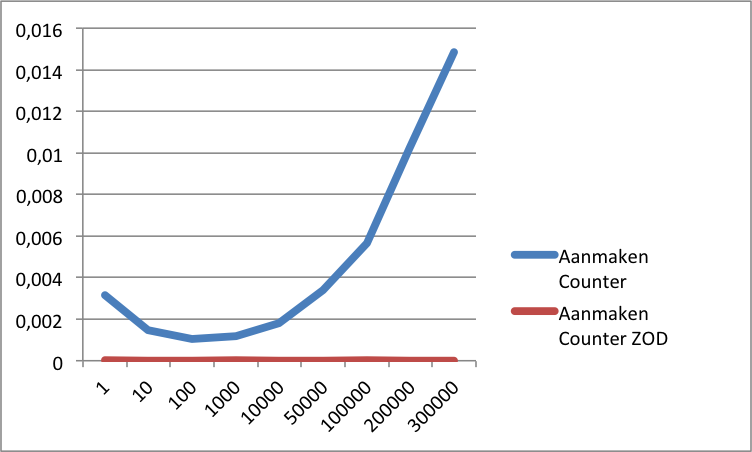
\includegraphics[scale=1.0]{Afbeeldingen/Evaluatie/AanmakenCounter}
  \caption{Grafiek vergelijking tijden aanmaken van een Counter.}
  \label{fig:GraphCounter}
\end{figure}

\begin{figure}[!h]
  \centering
  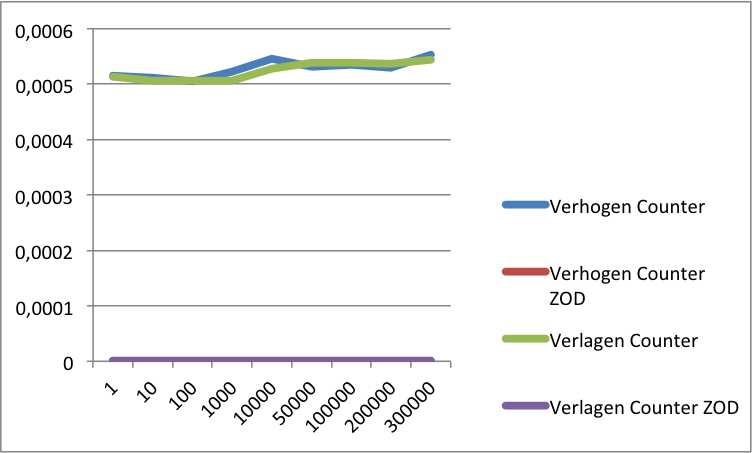
\includegraphics[scale=1.0]{Afbeeldingen/Evaluatie/VerhogenCounter}
  \caption{Grafiek vergelijking tijden verhogen van een Counter.}
  \label{fig:GraphCounterInc}
\end{figure}

\begin{figure}[!h]
  \centering
  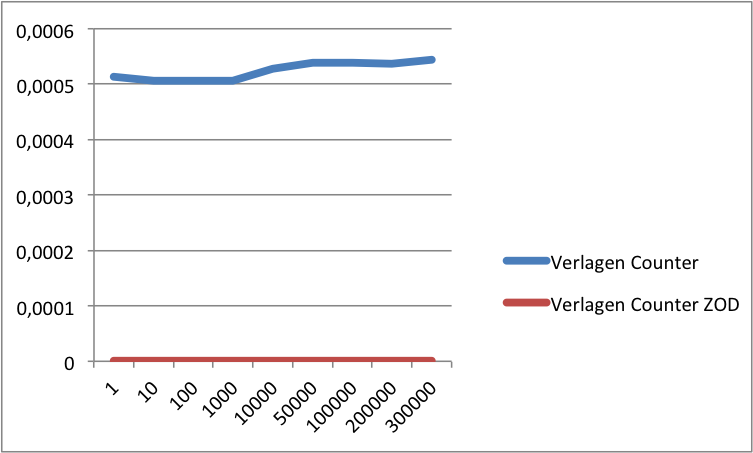
\includegraphics[scale=1.0]{Afbeeldingen/Evaluatie/VerlagenCounter}
  \caption{Grafiek vergelijking tijden verlagen van een Counter.}
  \label{fig:GraphCounterDec}
\end{figure}





\begin{table}[]
\centering
\begin{tabular}{|l|l|l|l|l|}
\hline
\# metingen   & Aanmaken    & Stop        & Aanmaken ZOD & Stop ZOD    \\ \hline
1         & 0,000342011 & 0,000580966 & 4,09013E-06  & 2,89679E-05 \\ \hline
10        & 0,000284296 & 0,000492996 & 1,91528E-06  & 5,6982E-06  \\ \hline
100       & 0,000298141 & 0,00049423  & 2,07685E-06  & 2,2608E-06  \\ \hline
1000      & 0,000297281 & 0,000522041 & 2,03055E-06  & 2,18725E-06 \\ \hline
10000     & 0,000740984 & 0,000527625 & 1,88986E-06  & 1,26034E-06 \\ \hline
50000     & 0,002660037 & 0,000536449 & 2,03353E-06  & 1,17797E-06 \\ \hline
100000    & 0,00515636  & 0,000544189 & 1,83201E-06  & 1,17261E-06 \\ \hline
200000    & 0,009800656 & 0,000575258 & 1,86301E-06  & 1,16086E-06 \\ \hline
300000    & 0,014302578 & 0,000522853 & 1,75735E-06  & 1,11202E-06 \\ \hline
Gemiddeld & 0,003764705 & 0,000532956 & 2,1654E-06   & 4,99977E-06 \\ \hline
\end{tabular}
\caption{Resultaten call tijd Timer (in seconden)}
\label{Table:Timer}
\end{table}

\begin{figure}[!h]
  \centering
  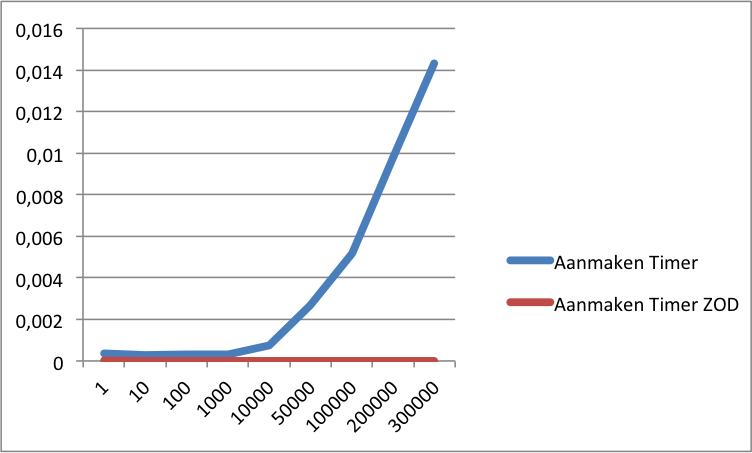
\includegraphics[scale=1.0]{Afbeeldingen/Evaluatie/AanmakenTimer}
  \caption{Grafiek vergelijking tijden aanmaken van een Timer.}
  \label{fig:GraphTimer}
\end{figure}

\begin{figure}[!h]
  \centering
  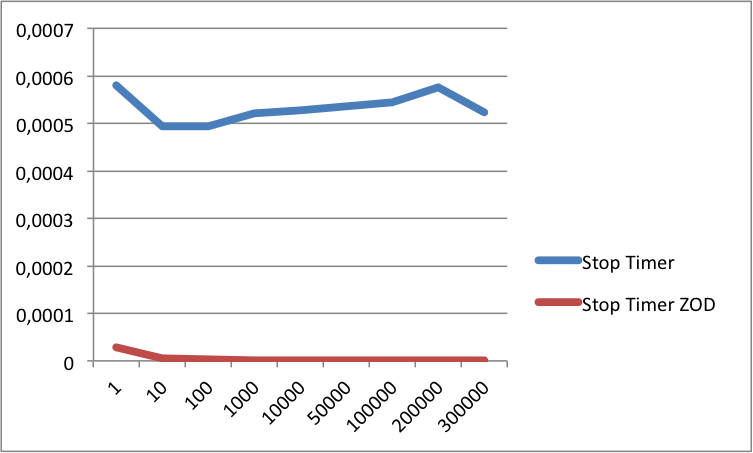
\includegraphics[scale=1.0]{Afbeeldingen/Evaluatie/StopTimer}
  \caption{Grafiek vergelijking tijden stoppen van een Timer.}
  \label{fig:GraphTimerStop}
\end{figure}


\begin{table}[]
\centering
\begin{tabular}{|l|l|l|l|l|}
\hline
\# metingen & Aanmaken    & Stop        & Aanmaken ZOD & Stop        \\ \hline
1           & 0,002120972 & 0,002666599 & 4,36699E-05  & 4,00181E-06 \\ \hline
10          & 0,000227898 & 0,002475894 & 3,0541E-05   & 1,69697E-06 \\ \hline
100         & 2,12032E-05 & 0,000657661 & 2,74795E-05  & 1,77817E-06 \\ \hline
1000        & 3,52955E-06 & 0,000614075 & 3,24672E-06  & 1,51634E-06 \\ \hline
10000       & 1,26566E-06 & 0,000587031 & 1,25878E-06  & 1,43751E-06 \\ \hline
50000       & 1,0892E-06  & 0,000584363 & 1,12291E-06  & 1,36487E-06 \\ \hline
100000      & 1,02262E-06 & 0,000574846 & 1,04058E-06  & 1,45262E-06 \\ \hline
200000      & 1,03471E-06 & 0,000565405 & 1,02583E-06  & 1,36E-06    \\ \hline
300000      & 1,0063E-06  & 0,000574488 & 1,01804E-06  & 1,4087E-06  \\ \hline
Gemiddeld   & 0,000264336 & 0,001033374 & 1,2267E-05   & 1,77967E-06 \\ \hline
\end{tabular}
\caption{Resultaten call tijd Timer met Aggregatie (in seconden)}
\label{Table:TimerAggregate}
\end{table}

\begin{figure}[!h]
  \centering
  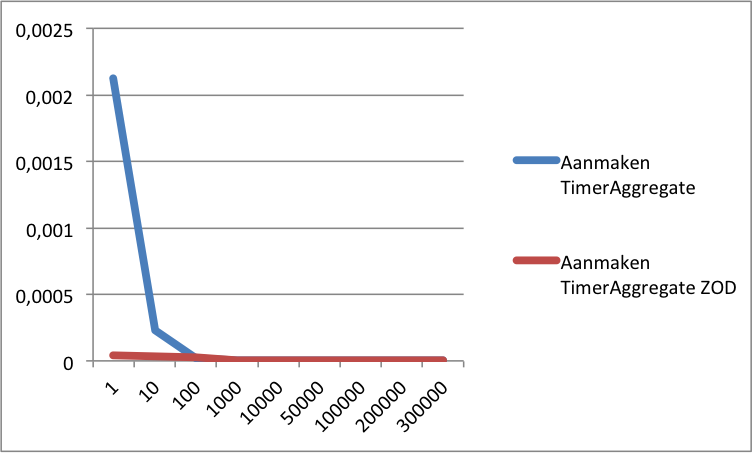
\includegraphics[scale=1.0]{Afbeeldingen/Evaluatie/AanmakenTimerAggregate}
  \caption{Grafiek vergelijking tijden aanmaken van een TimerAggregate object.}
  \label{fig:GraphTimerAggregate}
\end{figure}

\begin{figure}[!h]
  \centering
  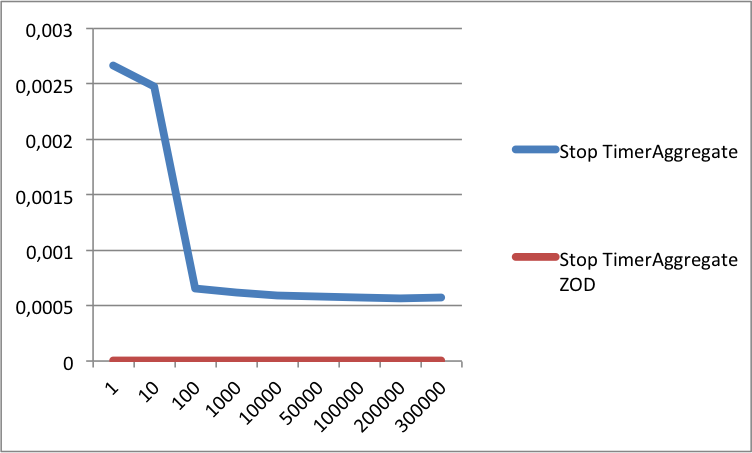
\includegraphics[scale=1.0]{Afbeeldingen/Evaluatie/StopTimerAggregate}
  \caption{Grafiek vergelijking tijden stoppen van een TimerAggregate object.}
  \label{fig:GraphTimerAggregateStop}
\end{figure}



\begin{table}[]
\centering
\begin{tabular}{|l|l|l|}
\hline
\# metingen & Aanmaken    & Aanmaken ZOD \\ \hline
1           & 0,002752006 & 4,21825E-06  \\ \hline
10          & 0,001020319 & 1,94199E-06  \\ \hline
100         & 0,001067632 & 2,11683E-06  \\ \hline
1000        & 0,001118987 & 2,89034E-06  \\ \hline
10000       & 0,001677553 & 2,00928E-06  \\ \hline
50000       & 0,003420756 & 1,86953E-06  \\ \hline
100000      & 0,005801659 & 1,86129E-06  \\ \hline
200000      & 0,010283894 & 1,85536E-06  \\ \hline
300000      & 0,014828387 & 1,8752E-06   \\ \hline
Gemiddeld   & 0,004663466 & 2,29312E-06  \\ \hline
\end{tabular}
\caption{Resultaten call tijd Histogram (in seconden)}
\label{Table:Histogram}
\end{table}

\begin{figure}[!h]
  \centering
  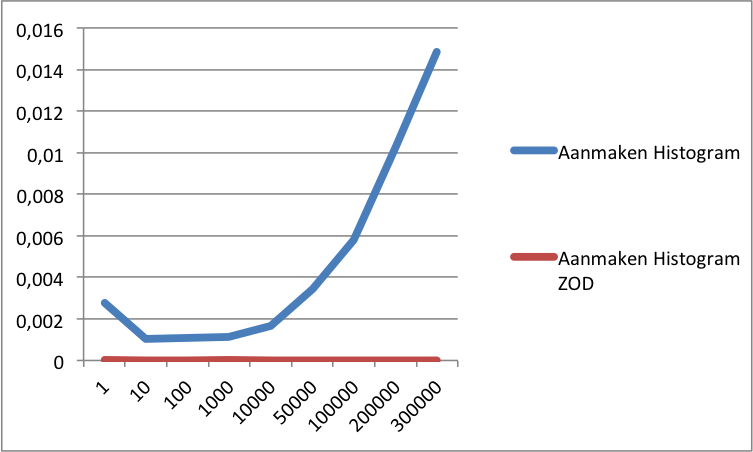
\includegraphics[scale=1.0]{Afbeeldingen/Evaluatie/AanmakenHistogram}
  \caption{Grafiek vergelijking tijden aanmaken van een Histogram.}
  \label{fig:GraphHistogram}
\end{figure}


\begin{table}[]
\centering
\begin{tabular}{|l|l|l|}
\hline
\# metingen & addEntry    & addEntry ZOD \\ \hline
1           & 0,002198004 & 3,99419E-06  \\ \hline
10          & 0,001131004 & 2,17136E-06  \\ \hline
100         & 0,001070941 & 2,1365E-06   \\ \hline
1000        & 0,001186648 & 2,36198E-06  \\ \hline
10000       & 0,001511716 & 2,28242E-06  \\ \hline
50000       & 0,003305941 & 2,04427E-06  \\ \hline
100000      & 0,005528791 & 2,23297E-06  \\ \hline
200000      & 0,010175614 & 1,88071E-06  \\ \hline
300000      & 0,015041323 & 1,89719E-06  \\ \hline
Gemiddeld   & 0,00457222  & 2,33351E-06  \\ \hline
\end{tabular}
\caption{Resultaten call tijd Meter (in seconden)}
\label{Table:Meter}
\end{table}

\begin{figure}[!h]
  \centering
  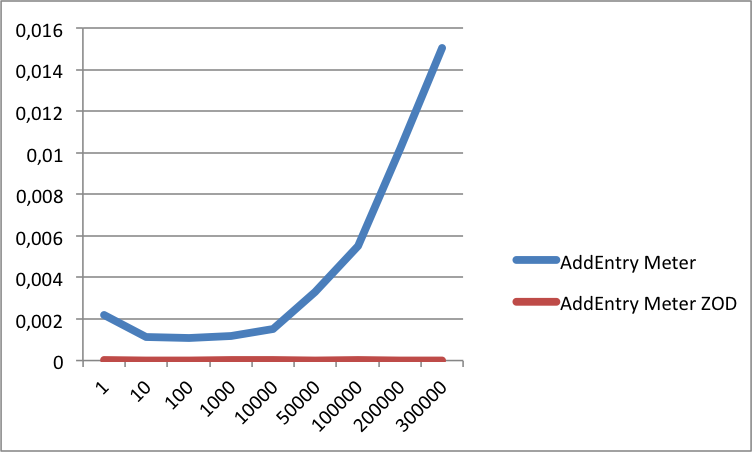
\includegraphics[scale=1.0]{Afbeeldingen/Evaluatie/AddEntryMeter}
  \caption{Grafiek vergelijking tijden addEntry van een Meter.}
  \label{fig:GraphMeter}
\end{figure}



\begin{table}[]
\centering
\begin{tabular}{|l|l|l|}
\hline
\# metingen & addEntry    & addEntry ZOD \\ \hline
1           & 0,025438964 & 4,48893E-05  \\ \hline
10          & 0,003257507 & 2,90151E-05  \\ \hline
100         & 0,000962322 & 6,39166E-06  \\ \hline
1000        & 0,000811738 & 1,56662E-06  \\ \hline
10000       & 0,000793704 & 1,18229E-06  \\ \hline
50000       & 0,000813867 & 1,15234E-06  \\ \hline
100000      & 0,000769992 & 1,0986E-06   \\ \hline
200000      & 0,000618082 & 1,15231E-06  \\ \hline
300000      & 0,000561398 & 1,10977E-06  \\ \hline
Gemiddeld   & 0,003780842 & 9,72867E-06  \\ \hline
\end{tabular}
\caption{Resultaten call tijd Meter met Aggregatie (in seconden)}
\label{Table:MeterAggregate}
\end{table}

\begin{figure}[!h]
  \centering
  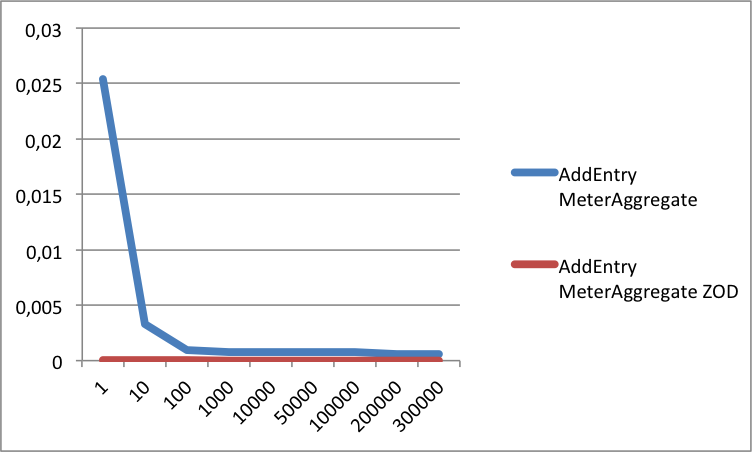
\includegraphics[scale=1.0]{Afbeeldingen/Evaluatie/AddEntryMeterAggregate}
  \caption{Grafiek vergelijking tijden addEntry van een MeterAggregate object.}
  \label{fig:GraphMeterAggregate}
\end{figure}


\begin{table}[]
\centering
\begin{tabular}{|l|l|l|}
\hline
\# metingen & Aanmaken    & Aanmaken ZOD \\ \hline
1           & 0,002469957 & 4,12756E-06  \\ \hline
10          & 0,001076302 & 1,95558E-06  \\ \hline
100         & 0,001117599 & 2,09727E-06  \\ \hline
1000        & 0,001157752 & 2,47002E-06  \\ \hline
10000       & 0,001552656 & 2,00483E-06  \\ \hline
50000       & 0,003327206 & 1,81246E-06  \\ \hline
100000      & 0,005833407 & 1,91939E-06  \\ \hline
200000      & 0,010283247 & 1,82617E-06  \\ \hline
300000      & 0,015243511 & 1,90657E-06  \\ \hline
Gemiddeld   & 0,004673515 & 2,23554E-06  \\ \hline
\end{tabular}
\caption{Resultaten call tijd Gauge (in seconden)}
\label{Table:Gauge}
\end{table}

\begin{figure}[!h]
  \centering
  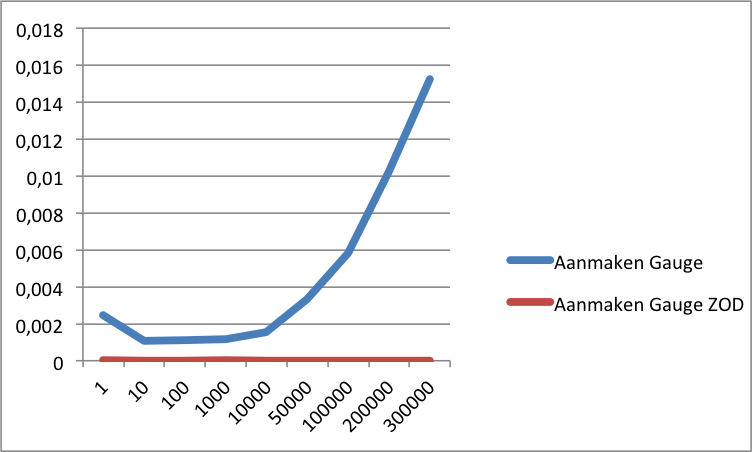
\includegraphics[scale=1.0]{Afbeeldingen/Evaluatie/AanmakenGauge}
  \caption{Grafiek vergelijking tijden aanmaken van een Gauge.}
  \label{fig:GraphGauge}
\end{figure}

\clearpage
\begin{table}[]
\centering
\begin{tabular}{|l|l|l|}
\hline
\# metingen & Aanmaken    & Aanmaken ZOD \\ \hline
1           & 0,018877983 & 0,002133965  \\ \hline
10          & 0,002148187 & 0,0004381    \\ \hline
100         & 0,00066519  & 0,000245582  \\ \hline
1000        & 0,000668403 & 0,000252874  \\ \hline
10000       & 0,001156017 & 0,000333561  \\ \hline
50000       & 0,002451678 & 0,001636235  \\ \hline
100000      & 0,004218748 & 0,003317311  \\ \hline
200000      & 0,007491983 & 0,006745731  \\ \hline
300000      & 0,011473117 & 0,01040852   \\ \hline
Gemiddeld   & 0,005461256 & 0,002834653  \\ \hline
\end{tabular}
\caption{Resultaten call tijd Gauge met Aggregatie (in seconden)}
\label{Table:GaugeAggregate}
\end{table}
\begin{figure}[!h]
  \centering
  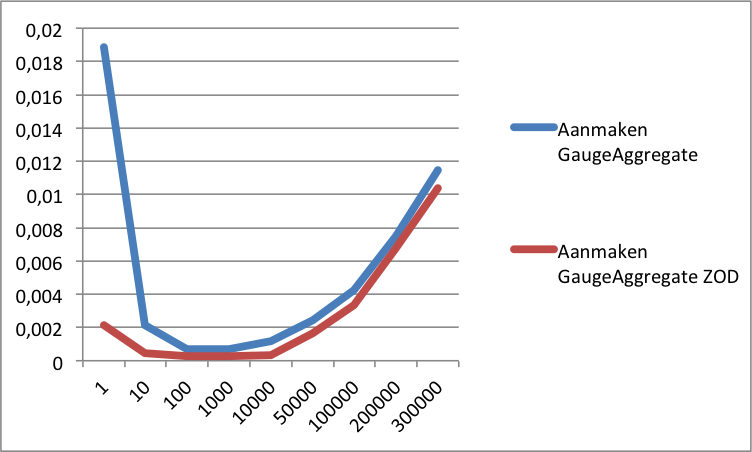
\includegraphics[scale=1.0]{Afbeeldingen/Evaluatie/AanmakenGaugeAggregate}
  \caption{Grafiek vergelijking tijden aanmaken van een GaugeAggregate.}
  \label{fig:GraphGaugeAggregate}
\end{figure}



\begin{table}[]
\centering
\begin{tabular}{|l|l|l|l|l|l|}
\hline
\#metingen/sec & 60 sec sync & 30 sec sync & 15 sec sync & 10 sec syn  & 5 sec sync \\ \hline
0              & 31,5632141  & 31,6737281  & 31,5281931  & 31,5672819  & 31,0382918 \\ \hline
1              & 31,5482895  & 31,5798341  & 31,5577123  & 31,5036609  & 31,2145193 \\ \hline
10             & 31,4920183  & 31,5852394  & 31,1482867  & 31,2389401  & 31,2015632 \\ \hline
20             & 30,9340218  & 30,9576821  & 30,8974831  & 30,91473821 & 30,7183928 \\ \hline
50             & 29,8320184  & 29,3209473  & 29,3382103  & 29,1371842  & 27,0873822 \\ \hline
100            & 20,8572947  &             &             &             &            \\ \hline
1000           & 9,3930281   &             &             &             &            \\ \hline
\end{tabular}
\caption{Resultaten metingen van het aanmaken van een Counter (in FPS)}
\label{Table:FPS}
\end{table}


\begin{table}
    \begin{tabular}{|l|l|l|l|l|l|}
        \hline
        \#metingen/sec & 60 sec sync & 30 sec sync & 15 sec sync & 10 sec syn & 5 sec sync \\ \hline
        0              & 31,1820647  & 31,8803964  & 31,3142858  & 31,6800421 & 31,22479   \\ \hline
        1              & 31,0432074  & 31,0152085  & 31,2826062  & 31,6564528 & 31,6203637 \\ \hline
        10             & 31,0542531  & 31,1544302  & 31,6991781  & 31,5175955 & 31,7503975 \\ \hline
        20             & 31,3124629  & 31,3124629  & 31,3124629  & 31,3124629 & 31,3124629 \\ \hline
        50             & 31,3699147  & 31,0174307  & 31,1349254  & 31,1842869 & 31,41264   \\ \hline
        100            & 31,2135833  & 31,222065   & 31,1640447  & 31,1833848 & 31,1436048 \\ \hline
        1000           & 30,2901981  & 30,2194739  & 30,2063641  & 30,1752    & 30,1750657 \\
        \hline
    \end{tabular}
\caption{Resultaten metingen van het stoppen van een Timer zonder opslaan op harde schijf (in FPS)}
\label{Table:FPSZOD}
\end{table}



\begin{figure}[!h]
  \centering
  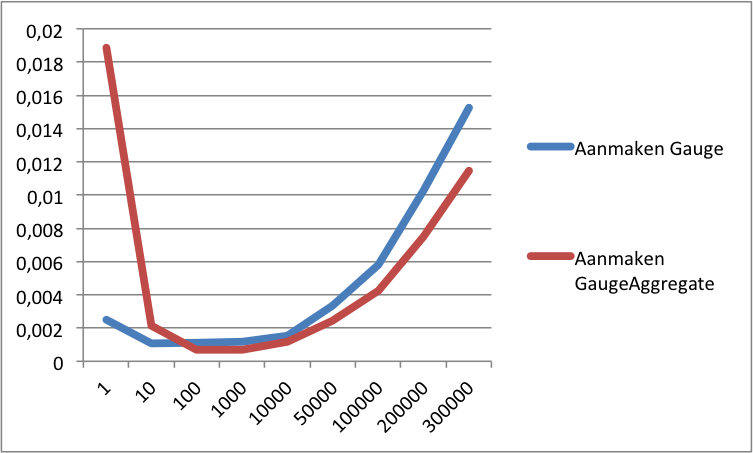
\includegraphics[scale=1.0]{Afbeeldingen/Evaluatie/GaugeVSAggregate}
  \caption{Grafiek vergelijking tussen het aanmaken van een Gauge en een GaugeAggregate object.}
  \label{fig:GaugeVSAggregate}
\end{figure}

\begin{figure}[!h]
  \centering
  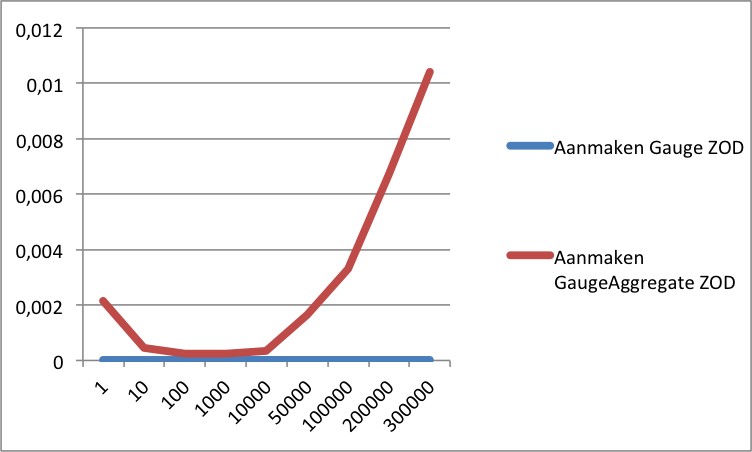
\includegraphics[scale=1.0]{Afbeeldingen/Evaluatie/GaugeVSAggregateZOD}
  \caption{Grafiek vergelijking tussen het aanmaken van een Gauge en een GaugeAggregate object zonder opslaan op de harde schijf.}
  \label{fig:GaugeVSAggregateZOD}
\end{figure}

\begin{figure}[!h]
  \centering
  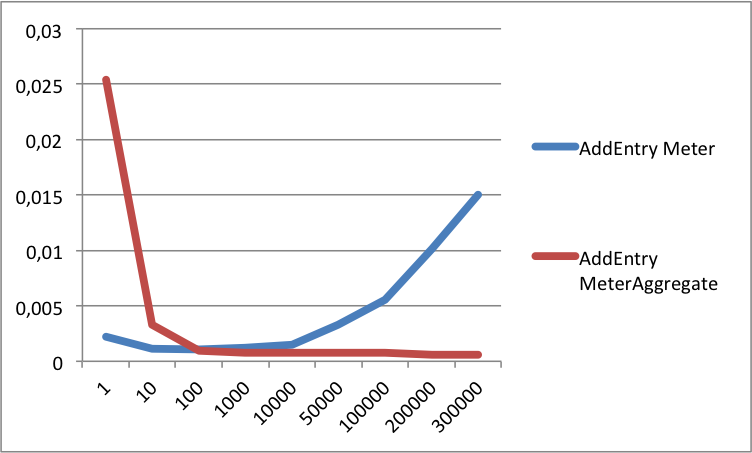
\includegraphics[scale=1.0]{Afbeeldingen/Evaluatie/MeterVSAggregate}
  \caption{Grafiek vergelijking tussen het aanmaken van een Meter en een MeterAggregate object.}
  \label{fig:MeterVSAggregate}
\end{figure}

\begin{figure}[!h]
  \centering
  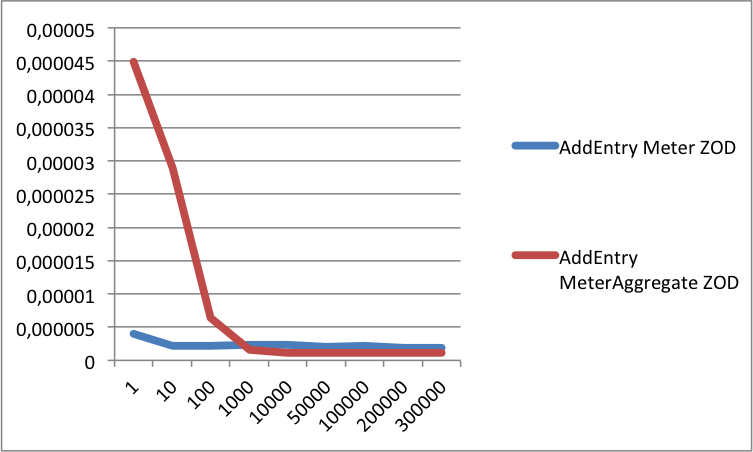
\includegraphics[scale=1.0]{Afbeeldingen/Evaluatie/MeterVSAggregateZOD}
  \caption{Grafiek vergelijking tussen het aanmaken van een Meter en een MeterAggregate object zonder opslaan op de harde schijf.}
  \label{fig:MeterVSAggregateZOD}
\end{figure}

\begin{figure}[!h]
  \centering
  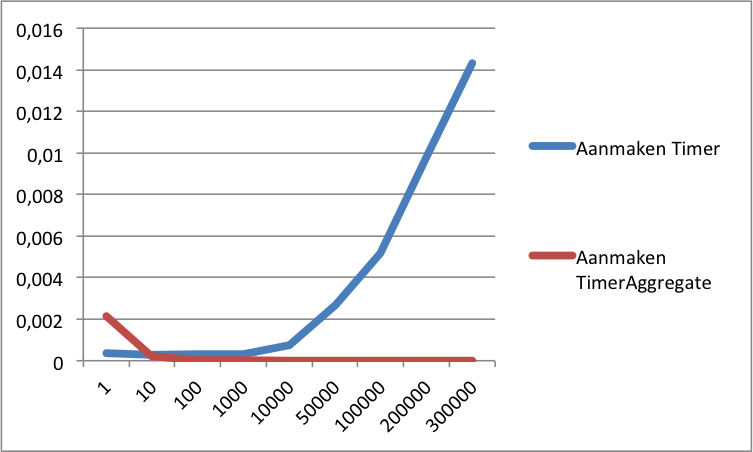
\includegraphics[scale=1.0]{Afbeeldingen/Evaluatie/TimerVSAggregate}
  \caption{Grafiek vergelijking tussen het aanmaken van een Timer en een TimerAggregate object.}
  \label{fig:TimerVSAggregate}
\end{figure}

\begin{figure}[!h]
  \centering
  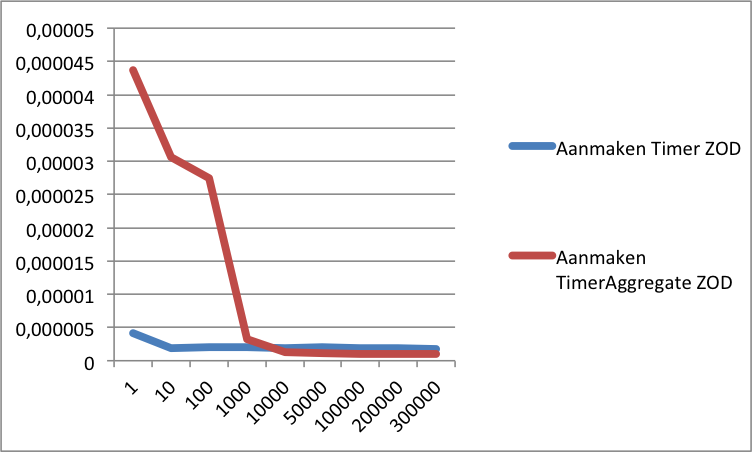
\includegraphics[scale=1.0]{Afbeeldingen/Evaluatie/TimerVSAggregateZOD}
  \caption{Grafiek vergelijking tussen het aanmaken van een Timer en een TimerAggregate object zonder opslaan op de harde schijf.}
  \label{fig:TimerVSAggregateZOD}
\end{figure}

\begin{figure}[!h]
  \centering
  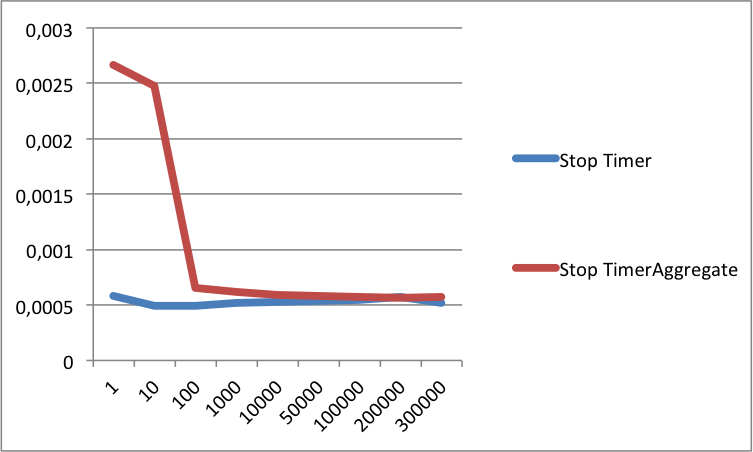
\includegraphics[scale=1.0]{Afbeeldingen/Evaluatie/StopVSTimerAggregate}
  \caption{Grafiek vergelijking tussen het aanroepen van de stop methode op een Timer en het aanroepen van de stop methode op een TimerAggregate object.}
  \label{fig:StopVSTimerAggregate}
\end{figure}

\begin{figure}[!h]
  \centering
  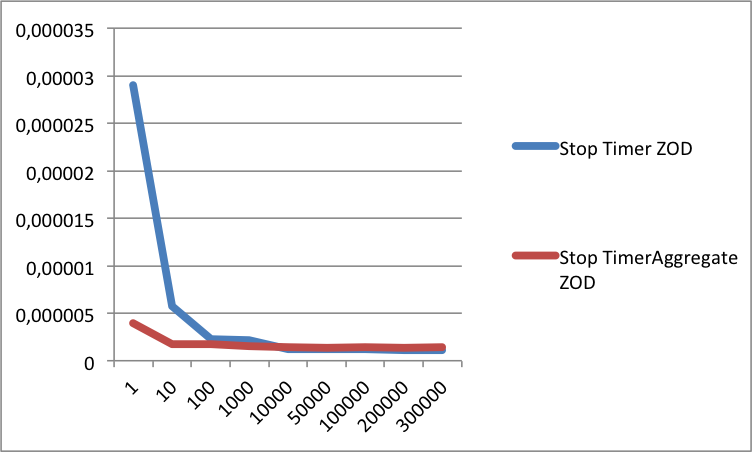
\includegraphics[scale=1.0]{Afbeeldingen/Evaluatie/StopVSTimerAggregateZOD}
  \caption{Grafiek vergelijking tussen het aanroepen van de stop methode op een Timer en het aanroepen van de stop methode op een TimerAggregate object zonder opslaan op de harde schijf..}
  \label{fig:StopVSTimerAggregateZOD}
\end{figure}



%%% Local Variables: 
%%% mode: latex
%%% TeX-master: "masterproef"
%%% End: 
